\documentclass[11pt]{article}

\usepackage[margin=1in]{geometry}
\usepackage{graphicx}
\usepackage{booktabs}
\usepackage{amsmath}
\usepackage{float}
\usepackage[hidelinks]{hyperref}
\usepackage[numbers]{natbib}

% Works both locally (figures in ../figures) and on Overleaf (figures/ next to main.tex)
\graphicspath{{figures/}{../figures/}}

\title{Detecting Mining-Driven Deforestation in Central India with a Transfer-Learned Land-Cover Classifier: A Two-Site Study Validated Against Global Forest Watch}
\author{Arnav \\ Plaksha University \\ \texttt{arnavmandre007@gmail.com}}
\date{October 2026}

\begin{document}
\maketitle

\begin{abstract}
Open-pit coal mining is clearing forest in central India, and free satellite imagery makes it possible in principle to watch this happen. This project tests whether a lightweight, off-the-shelf approach can detect such clearing. A ResNet50 network pretrained on ImageNet was fine-tuned on EuroSAT, a dataset of 27,000 European Sentinel-2 image patches in ten land-cover classes, reaching 97.70\% accuracy on a held-out test set. The classifier was then applied to Sentinel-2 imagery of a 16 $\times$ 16 km area around the Parsa East and Kanta Basan coal mine in Hasdeo Arand, Chhattisgarh, for February 2019 and February 2025. Each image was divided into 625 patches of 640 m, and patches were flagged as deforested either when their label changed from Forest to another class (method A) or when their predicted Forest probability fell by at least 0.5 (method B). Against Global Forest Watch tree-cover-loss data for 2019--2024, both methods found 82\% of the patches with substantial loss, with precision of 47\% (A) and 53\% (B). Applied without changes to a second site, the Talabira II \& III coal mine in Odisha, the methods reached a recall of 75\% and precisions of 50\% and 55\%. The approach reliably locates large clearings but produces many false alarms, mainly from hill shadows, clouds, mixed patches and the absence of a mining class, and it overestimates cleared area by a factor of 3.7. It is therefore better suited to flagging candidate areas for inspection than to measuring forest loss.
\end{abstract}

\section{Introduction}

Forests are being lost worldwide at a rate that satellite monitoring has made measurable: global, 30 m maps of annual tree-cover change built from the Landsat archive \citep{hansen2013} now underpin tools such as Global Forest Watch (GFW). In India, a visible driver of local forest loss is open-pit coal mining. Hasdeo Arand in Chhattisgarh, one of the largest contiguous dense forests in central India, overlies a major coalfield, and the Parsa East and Kanta Basan (PEKB) mine within it has expanded in recent years \citep{gem_pekb}. In Odisha, the Talabira II \& III mine drew national attention when tree felling for it began in December 2019 \citep{mongabay2019}.

Since 2015, the European Space Agency's Sentinel-2 satellites have imaged the whole land surface every few days at 10 m resolution, free of charge \citep{drusch2012}. Deep convolutional neural networks have proven effective at classifying land cover in such imagery; on the EuroSAT benchmark, built from Sentinel-2 patches across Europe, fine-tuned ImageNet networks exceed 98\% accuracy \citep{helber2019}. An open question for anyone wanting to use such a model in practice is how well it transfers: a model trained on European landscapes will see different vegetation, soils and lighting in tropical India.

This project asks: \emph{can a classifier trained only on European imagery detect mining-driven forest loss in India, and how far can its detections be trusted?} The contributions are:
\begin{enumerate}
    \item a reproducible pipeline that classifies Sentinel-2 imagery of two dates into land-cover maps and compares them;
    \item a quantitative validation of the detected changes against GFW tree-cover-loss data;
    \item a test on a second, independent site with all settings fixed in advance; and
    \item an analysis of the failure modes that limit this approach.
\end{enumerate}

\section{Data}

\subsection{EuroSAT}
EuroSAT \citep{helber2019} contains 27,000 RGB image patches from Sentinel-2, each 64 $\times$ 64 pixels at 10 m per pixel (640 m $\times$ 640 m on the ground). Each patch carries one of ten labels: Annual Crop, Forest, Herbaceous Vegetation, Highway, Industrial, Pasture, Permanent Crop, Residential, River and Sea/Lake. Classes contain between 2,000 and 3,000 patches. The dataset was split at random into training (21,600), validation (2,700) and test (2,700) sets using a fixed seed (42).

\subsection{Study areas and Sentinel-2 imagery}
Two sites were studied (Table~\ref{tab:scenes}): a 16 $\times$ 16 km window centred on the PEKB mine in Hasdeo Arand \citep{gem_pekb}, and a window of the same size centred on the Talabira II \& III mine \citep{gem_talabira}. Images were Sentinel-2 Level-2A (atmospherically corrected) true-colour products, retrieved from the Element 84 Earth Search catalogue. For each site, both dates were taken from the same Sentinel-2 tile so that pixels align exactly, and from the same season, to reduce seasonal differences in vegetation. At Hasdeo, dry-season scenes with less than 5\% cloud were used. At Talabira, many winter scenes were hazy, so the pair with the highest image contrast in the same season was chosen.

\begin{table}[H]
\centering
\caption{Study areas and Sentinel-2 scenes.}
\label{tab:scenes}
\begin{tabular}{lllll}
\toprule
Site & Centre (lat, lon) & Tile & Before & After \\
\midrule
Hasdeo Arand (PEKB) & 22.838$^\circ$N, 82.814$^\circ$E & 44QPL & 20 Feb 2019 & 8 Feb 2025 \\
Talabira II \& III & 21.735$^\circ$N, 83.989$^\circ$E & 44QRK & 24 Mar 2019 & 25 Mar 2025 \\
\bottomrule
\end{tabular}
\end{table}

\subsection{Reference data}
Validation used the Hansen Global Forest Change dataset, version 1.13 \citep{hansen2013}, which records, for each 30 m Landsat pixel, the year in which tree cover was lost (2001--2025). Loss in 2019--2024 was taken to have occurred between the two images. Loss recorded in 2025 was excluded because most of it occurred after the February and March 2025 images. The loss-year layer was reprojected onto each site's 10 m image grid using nearest-neighbour resampling.

\section{Methods}

\subsection{Classifier}
A ResNet50 \citep{he2016} pretrained on ImageNet \citep{deng2009} was adapted by replacing its final 1,000-class layer with a 10-class layer. Images were resized from 64 to 224 pixels and normalised with the ImageNet channel means and standard deviations. Training images were augmented with random horizontal and vertical flips, which preserve meaning for overhead imagery. Training ran in two stages. In stage 1, all pretrained layers were frozen and only the new layer was trained for 5 epochs with Adam \citep{kingma2015} at a learning rate of $10^{-3}$. In stage 2, all layers were unfrozen and trained for 5 more epochs at $10^{-4}$. The model with the highest validation accuracy was kept. Training used a batch size of 64 and bfloat16 mixed precision in PyTorch \citep{paszke2019} on a laptop RTX 5060 GPU, taking about one minute per epoch.

\subsection{Change detection}
Each 1,600 $\times$ 1,600 pixel window was cut into a 25 $\times$ 25 grid of 64 $\times$ 64 patches, the same size as EuroSAT patches. Each patch covers 0.41 km$^2$, giving 625 patches per date. Every patch was classified, giving a predicted class and a probability for each class. Two change rules were compared:
\begin{itemize}
    \item \textbf{Method A (label change):} a patch is flagged if it was classified as Forest in the first image and as any other class in the second.
    \item \textbf{Method B (probability drop):} a patch is flagged if its Forest probability fell by at least 0.5:
    \begin{equation}
    \Delta p = p_{\text{Forest}}^{\text{before}} - p_{\text{Forest}}^{\text{after}} \geq 0.5 .
    \end{equation}
\end{itemize}
Method B was introduced because a label can flip on a tiny change in probability (from 51\% to 49\%), while a large drop in probability may not change the label.

Re-colouring the Indian images to match EuroSAT's average colour and contrast was also tried. Because it made the land-cover maps markedly worse, it was not used.

\subsection{Validation}
For each patch, the fraction of its pixels with GFW loss in 2019--2024 was computed. A patch was counted as truly deforested if this fraction was at least 10\%. Each patch then falls into one of four categories: true positive (TP, flagged and deforested), false positive (FP, flagged but not deforested), false negative (FN, deforested but not flagged), or true negative. Performance is reported as
\begin{equation}
\text{precision} = \frac{TP}{TP+FP}, \quad \text{recall} = \frac{TP}{TP+FN}, \quad F_1 = \frac{2 \cdot \text{precision} \cdot \text{recall}}{\text{precision}+\text{recall}}.
\end{equation}
Accuracy is not reported, because almost all patches are true negatives and accuracy would be high even for a detector that never flags anything.

The cut-off of 0.5 in method B was selected at Hasdeo while comparing against GFW, so the Hasdeo results for method B are optimistic. To obtain an unbiased estimate, all settings (patch size, model, both rules, the 0.5 cut-off and the 10\% threshold) were then fixed and applied unchanged to Talabira.

\section{Results}

\subsection{Classifier accuracy}
On the 2,700 held-out EuroSAT test images, the classifier reached 97.70\% accuracy (62 errors) and a macro-averaged $F_1$ of 97.65\%. Forest was the best-recognised class ($F_1$ = 99.5\%; precision 99.7\%, recall 99.3\%) and Permanent Crop the worst ($F_1$ = 95.3\%). The most frequent confusion was Herbaceous Vegetation predicted as Permanent Crop (12 images), followed by Permanent Crop as Annual Crop (6) and River as Highway (5) (Figure~\ref{fig:cm}). Mean confidence was 99.0\% on correct predictions and 79.9\% on errors. Keeping only predictions with confidence of at least 90\% retained 95.7\% of test images and raised accuracy on them to 99.26\%.

\begin{figure}[H]
\centering
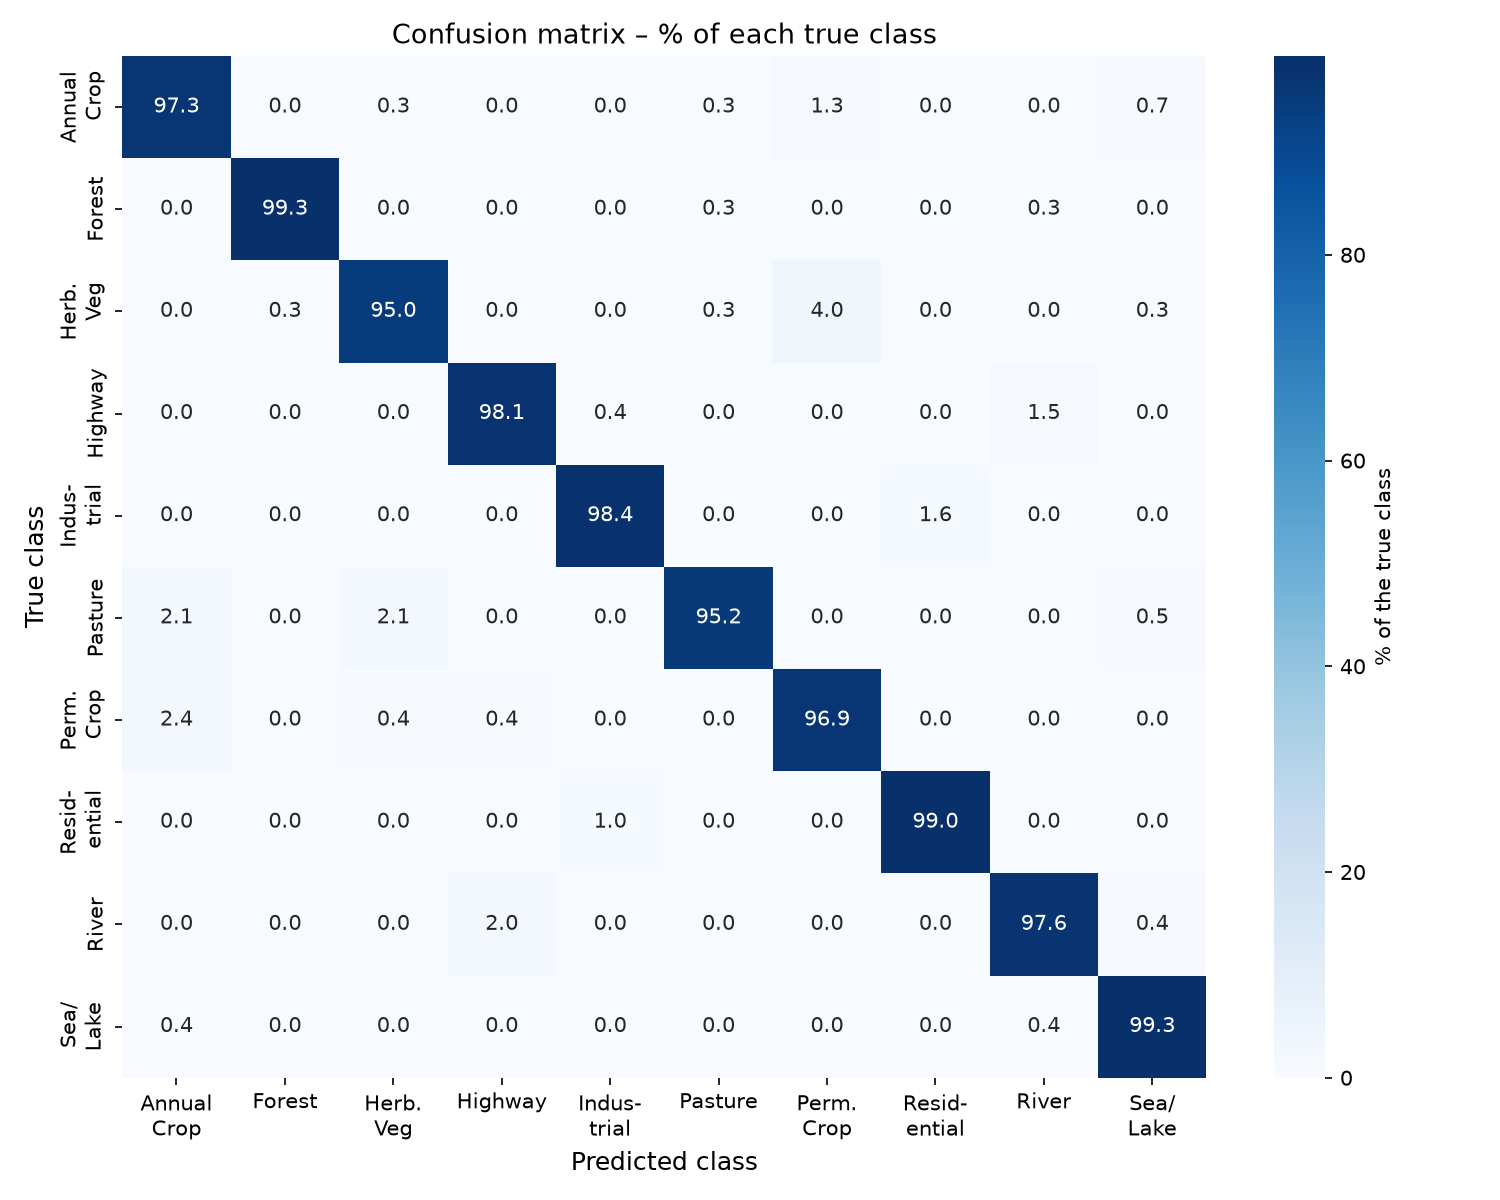
\includegraphics[width=0.68\linewidth]{confusion_matrix_percent.png}
\caption{Confusion matrix on the EuroSAT test set, as a percentage of each true class. Off-diagonal cells are errors.}
\label{fig:cm}
\end{figure}

\subsection{Land cover and change at Hasdeo Arand}
Between the two images, the PEKB pit widened substantially and a new clearing appeared north-west of it (Figure~\ref{fig:hasdeo}). The model classified most of the window as Forest (418 of 625 patches in 2019), and mean confidence on the Indian patches (86--87\%) was lower than on EuroSAT. With no mining class available, the model labelled the 2025 pit mainly as Herbaceous Vegetation, Sea/Lake, Highway or River. GFW recorded 2.09 km$^2$ of tree-cover loss in the window for 2019--2024, mostly in 2023 (0.48 km$^2$) and 2024 (1.48 km$^2$), concentrated around the mine. A further 1.50 km$^2$ was recorded for 2025.

\begin{figure}[H]
\centering
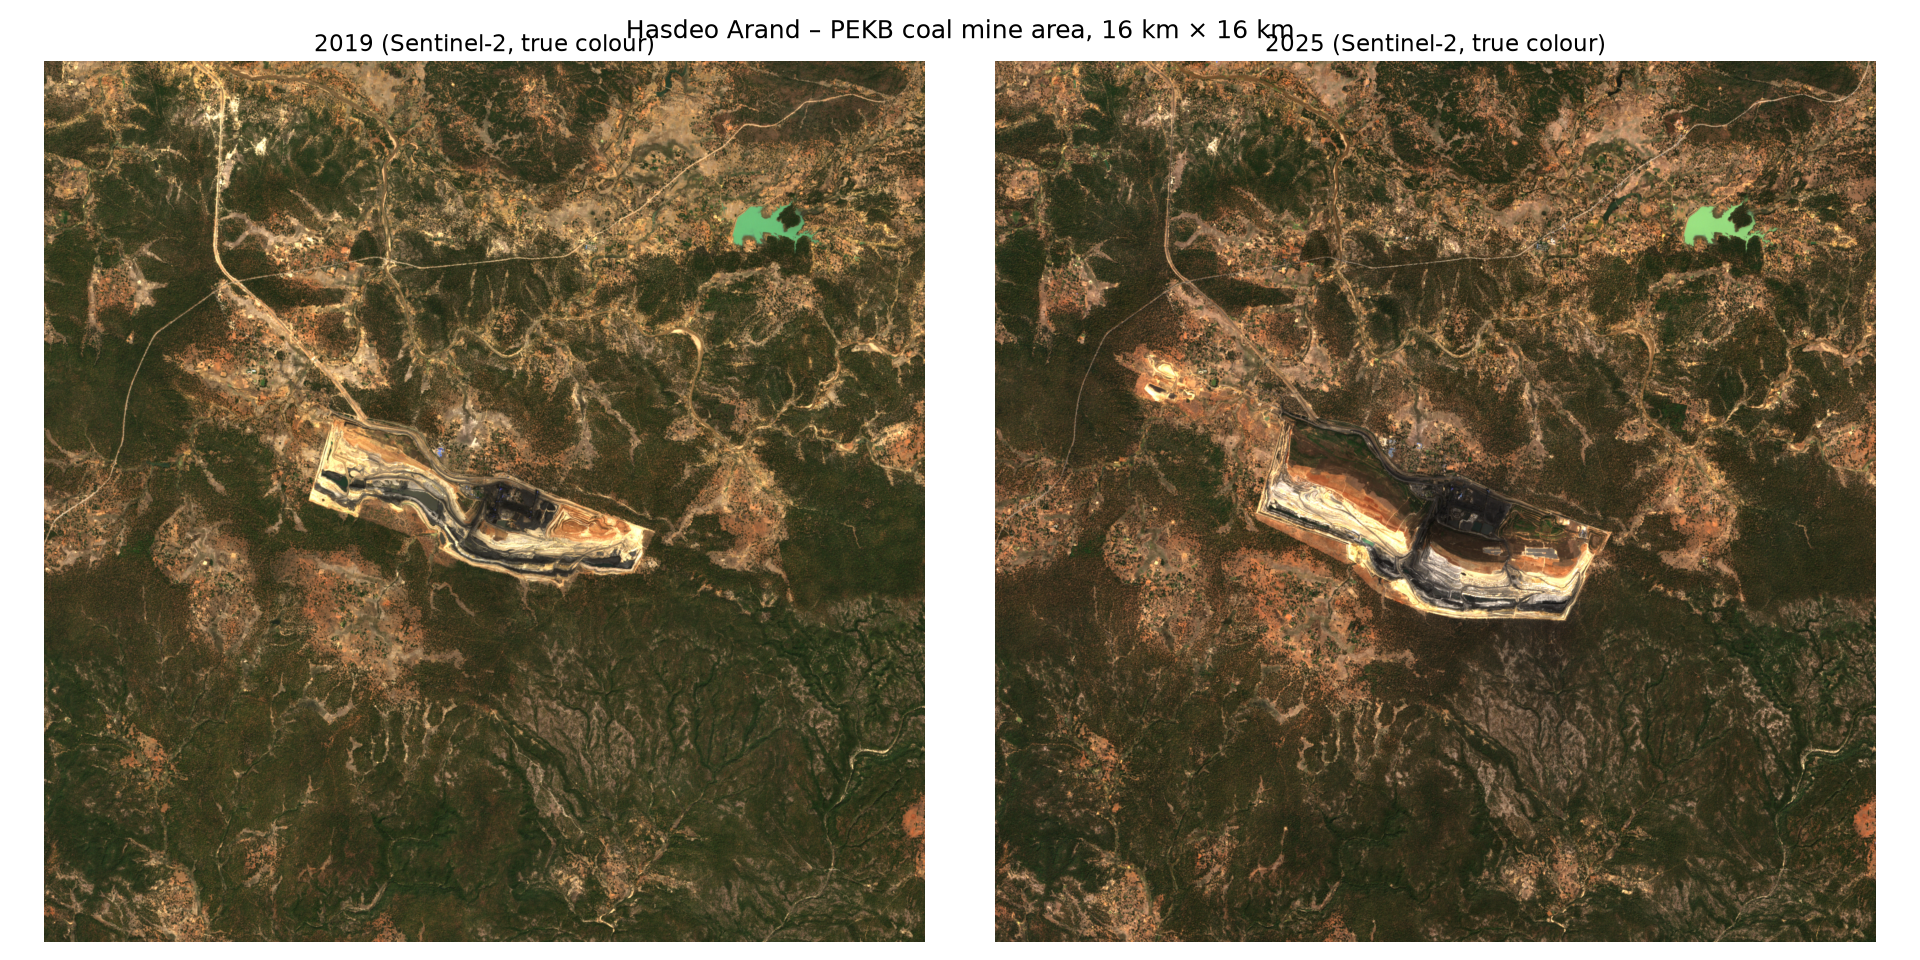
\includegraphics[width=\linewidth]{hasdeo_2019_vs_2025.png}
\caption{Sentinel-2 true-colour images of the 16 $\times$ 16 km Hasdeo Arand window in February 2019 (left) and February 2025 (right). The PEKB open pit is at the centre.}
\label{fig:hasdeo}
\end{figure}

\subsection{Agreement with Global Forest Watch}
At Hasdeo, 11 patches met the 10\% loss threshold. Method A flagged 19 patches, of which 9 matched (precision 47\%, recall 82\%). Method B flagged 17, also with 9 matches (precision 53\%, recall 82\%). Correct detections lay along the expanding pit and at the north-west clearing. The largest group of false alarms lay in the far south, in unchanged, shadowed forest that the model labelled Sea/Lake (Figure~\ref{fig:validation}). The same label comparison also showed 58 patches changing from non-forest to Forest. Because forest cannot regrow over whole 640 m patches in six years, these show the level of label noise between the two dates.

\begin{figure}[H]
\centering
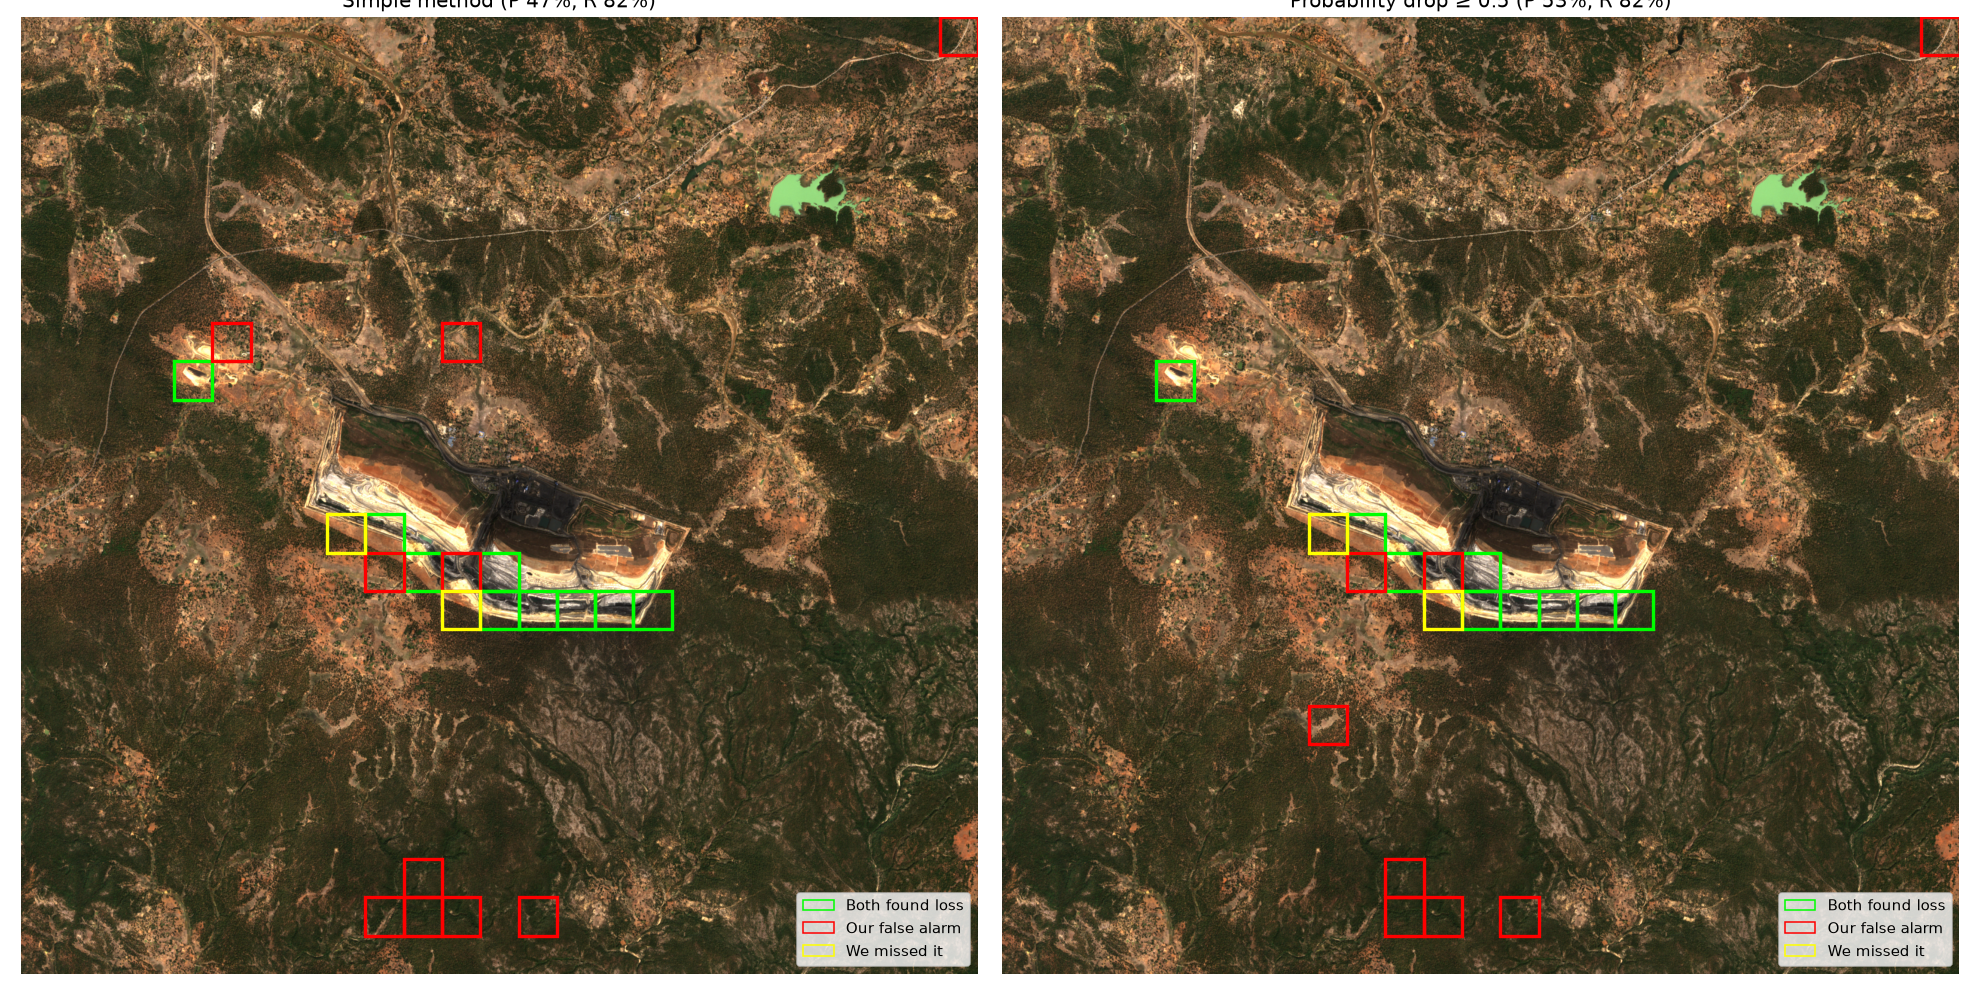
\includegraphics[width=\linewidth]{validation_map_comparison.png}
\caption{Detected change at Hasdeo compared with GFW, drawn on the 2025 image, for method A (left) and method B (right). Green: flagged by both; red: flagged by the model only (false alarm); yellow: GFW loss missed by the model.}
\label{fig:validation}
\end{figure}

At Talabira, with all settings fixed in advance, 8 patches met the loss threshold. Method A flagged 12 patches (6 correct: precision 50\%, recall 75\%) and method B flagged 11 (6 correct: precision 55\%, recall 75\%). Table~\ref{tab:results} and Figure~\ref{fig:sites} summarise both sites. GFW recorded most of Talabira's 2019--2024 loss in 2023 (0.89 km$^2$) and 2024 (0.67 km$^2$).

\begin{table}[H]
\centering
\caption{Patch-level agreement with GFW (a patch is lost if at least 10\% of it shows GFW loss in 2019--2024). $^\dagger$Cut-off chosen at this site.}
\label{tab:results}
\begin{tabular}{llrrrrrr}
\toprule
Site & Method & TP & FP & FN & Precision & Recall & $F_1$ \\
\midrule
Hasdeo   & A: label change               & 9 & 10 & 2 & 47\% & 82\% & 60\% \\
Hasdeo   & B: $\Delta p \geq 0.5^\dagger$ & 9 & 8  & 2 & 53\% & 82\% & 64\% \\
Talabira & A: label change               & 6 & 6  & 2 & 50\% & 75\% & 60\% \\
Talabira & B: $\Delta p \geq 0.5$        & 6 & 5  & 2 & 55\% & 75\% & 63\% \\
\bottomrule
\end{tabular}
\end{table}

\begin{figure}[H]
\centering
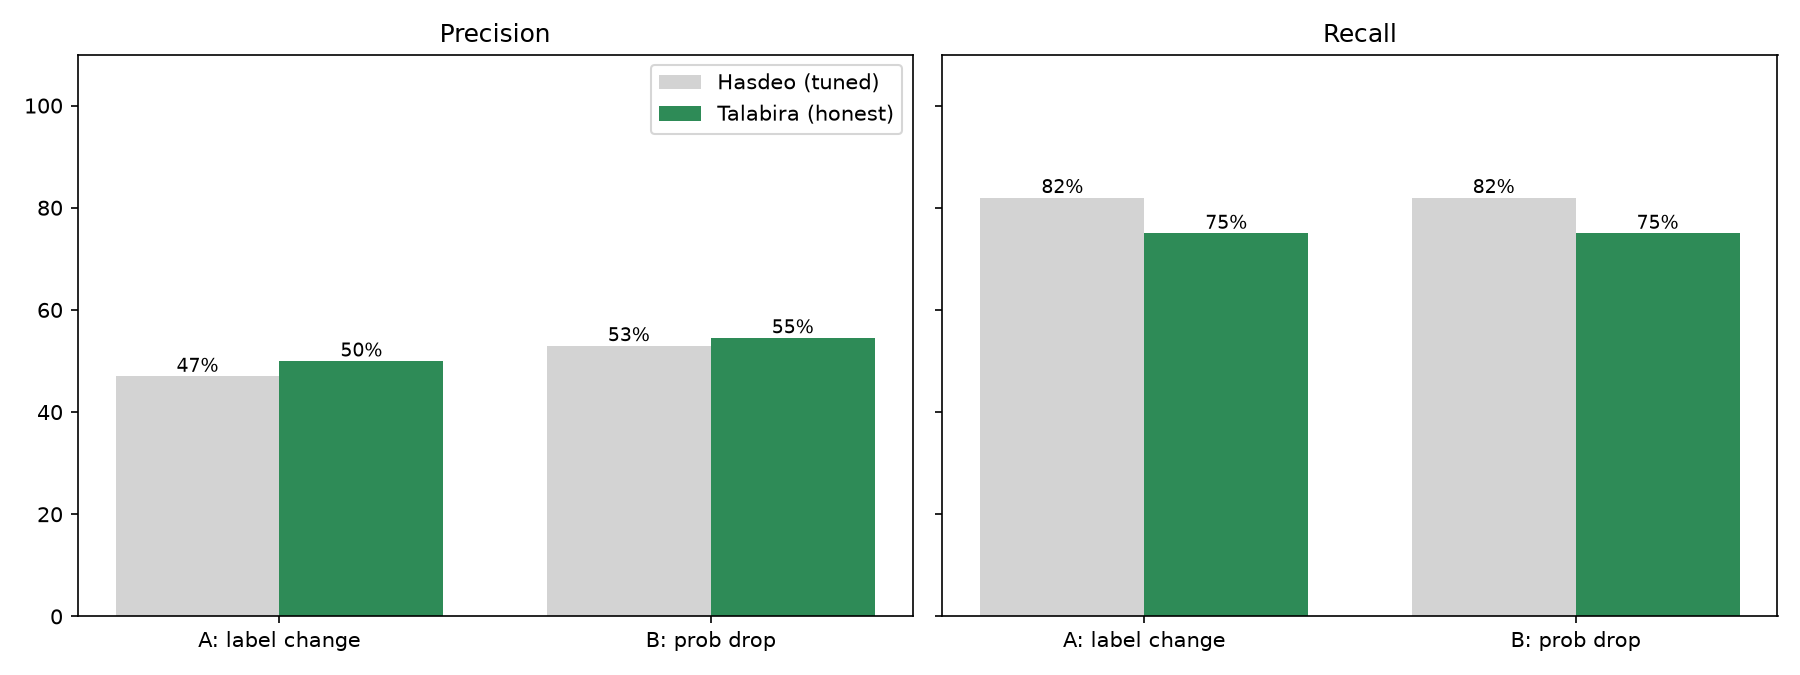
\includegraphics[width=0.8\linewidth]{hasdeo_vs_talabira.png}
\caption{Precision and recall of both methods at Hasdeo (cut-off tuned there) and Talabira (settings fixed in advance).}
\label{fig:sites}
\end{figure}

The results were not sensitive to the exact threshold used to define a lost patch. At Hasdeo, method A's recall rose from 55\% to 100\% as the threshold increased from 1\% to 50\% of a patch, while precision fell from 58\% to 21\%. Recall stayed at 73\% or higher for every threshold of 5\% and above.

\subsection{Area estimate}
Counting each flagged patch as fully cleared, method A estimated 7.8 km$^2$ of loss at Hasdeo against 2.09 km$^2$ from GFW, an overestimate by a factor of 3.7. The correctly flagged patches nonetheless contained 1.71 km$^2$, or 82\%, of all GFW loss in the window.

\section{Discussion}

The results answer the central question with a qualified yes. A classifier trained only on European images, applied with no Indian training data, located three-quarters or more of the substantially cleared patches at two mining sites in different states. The near-identical scores at Talabira, where nothing was tuned, indicate that this is a property of the method rather than of the Hasdeo data. However, roughly half of all alerts were false, so the method is better treated as a way to \emph{direct attention} than as a measurement.

The errors have identifiable causes. First, \textbf{domain shift}: average EuroSAT forest colour is bluish (RGB $\approx$ 39, 63, 75), while dry-season forest at Hasdeo is brown (RGB $\approx$ 69, 65, 38). This difference stems partly from geography and season and partly from processing, since EuroSAT was built from imagery without atmospheric correction while this study used corrected imagery. Lower confidence on Indian patches is one sign of this shift. A simple colour-matching correction made results worse, apparently because stretching contrast exaggerated canopy texture. Second, \textbf{missing classes}: with no mining or bare-ground class, the model had to name open pits after the nearest familiar class, often Sea/Lake for dark coal. Third, \textbf{shadows and clouds}: dark, shadowed slopes at Hasdeo and small clouds and their shadows at Talabira were labelled as water, producing confident false alarms. Fourth, \textbf{mixed patches}: a 640 m patch must receive a single label, so partially cleared patches can flip either way. This explains both the label noise (58 spurious forest gains at Hasdeo) and the 3.7-fold overestimate of area.

A notable finding is that \textbf{confidence did not transfer}. On EuroSAT, discarding low-confidence predictions raised accuracy above 99\%. At Hasdeo, however, some false alarms were made with more than 90\% confidence on both dates, while real detections at the mine edge often had low confidence, because the model had never seen a mine. A confidence filter tuned on the training domain may therefore discard true detections in a new domain.

The reference data has limits of its own. GFW records loss of tree cover only, so clearing of scrub or fields, which the model may flag as change, does not appear in it. Its loss years also do not always match reported events: at Talabira, felling was reported from December 2019, but GFW places most loss in 2023--2024. Some false positives may therefore be real land-cover change, and the precision figures should be read as lower bounds on usefulness rather than exact error rates.

Methodologically, the two-site design addresses a common pitfall. Choosing a decision threshold while scoring against the same reference data inflates performance. Fixing the method at Hasdeo and testing it unchanged at Talabira gives a fairer estimate, and method B's small advantage held at both sites.

The study has further limitations. Only two dates per site were used, so seasonal and atmospheric differences between them are confounded with real change. Only RGB bands were used, even though Sentinel-2 provides 13 bands, including near-infrared bands that separate vegetation from bare ground. The two sites are both coal mines and are small samples (11 and 8 lost patches), so the precision and recall estimates are uncertain. Finally, clearing recorded by GFW for 2025 at Hasdeo (1.50 km$^2$) fell after the second image and could not be detected.

Natural next steps are: using a 2026 image to capture 2025 clearing; adding a mining or bare-ground class; masking clouds and shadows; using all 13 spectral bands; using smaller patches or per-pixel segmentation for area estimates; fine-tuning on labelled Indian imagery; and testing on non-mining deforestation, such as shifting cultivation in north-east India.

\section{Conclusion}

A ResNet50 classifier fine-tuned on EuroSAT reached 97.7\% accuracy on European test data and, applied to Sentinel-2 images of two Indian coal mines, located 75--82\% of the patches where Global Forest Watch recorded substantial tree-cover loss in 2019--2024. About half of its alerts were false, and patch-based counting overstated cleared area 3.7-fold. Comparing Forest probabilities rather than labels gave a modest, consistent improvement that held on an untuned second site. Built entirely from free data and a laptop GPU, the approach is useful for flagging where clearing is happening, but not, in its current form, for measuring how much.

\section*{Data and code availability}
All code, notebooks, figures and patch-level results are available at \url{https://github.com/arnavmandre/eurosat-deforestation}. EuroSAT, Sentinel-2 imagery (via Element 84 Earth Search) and the Hansen Global Forest Change data are freely available.

\section*{AI use}
The code, the Jupyter notebooks and the text of this report were written with the help of an AI assistant (Claude, Anthropic; model Claude Opus 5.5; October 2026), working under the author's direction. The author set up the computing environment, ran every notebook, inspected the outputs and figures, and answered the analysis questions in each notebook. This report is a personal project write-up and has not been peer reviewed.

\bibliographystyle{plainnat}
\bibliography{references}

\end{document}
